

\section{DNS}
\subsection{Domain name resolver}
As you have a brand new server you are most probably have use a domain name resolver from a big company like Google, Cloudfare etc. But after the script you have your own resolver which is even better than the one which is by default configured. 
\subsubsection{BEFORE script}
Before running the script you get a C from \textbf{\textit{https://cmdns.dev.dns-oarc.net/} \cite{cmdns}}

\begin{figure}[H]
	\centering
	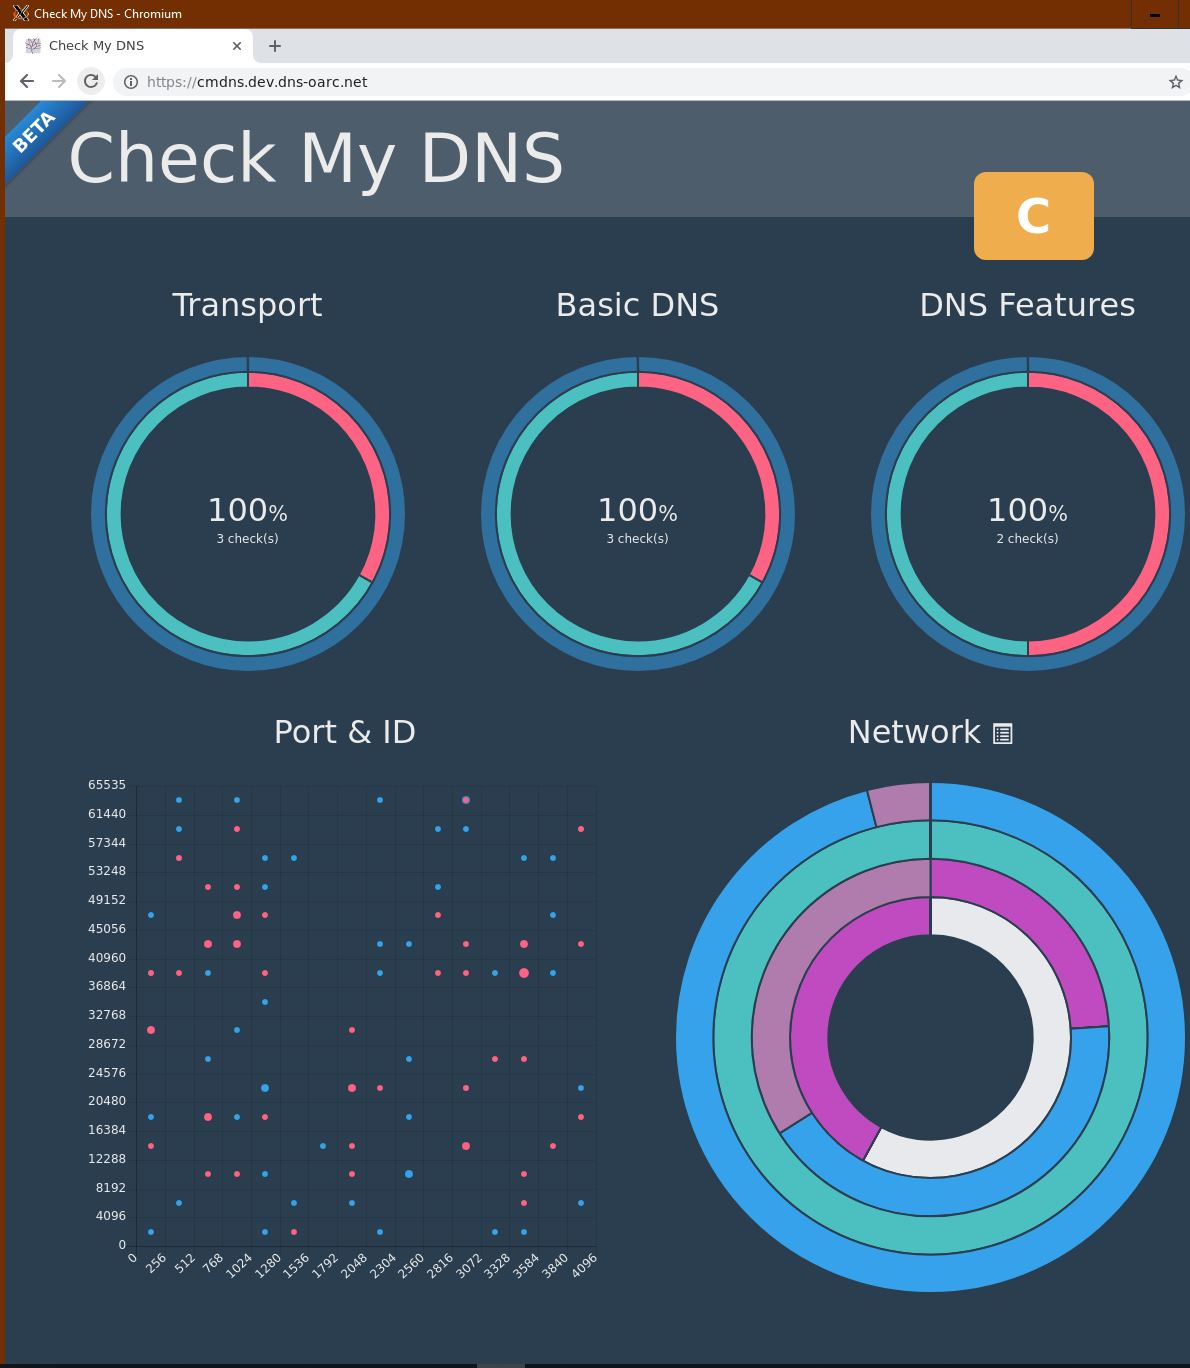
\includegraphics[width=0.6\linewidth]{pics/score_DNS1_before}
	\caption{Name resolver \textbf{BEFORE}}
	\label{fig:scoredns1before}
\end{figure}

\begin{figure}[H]
	\centering
	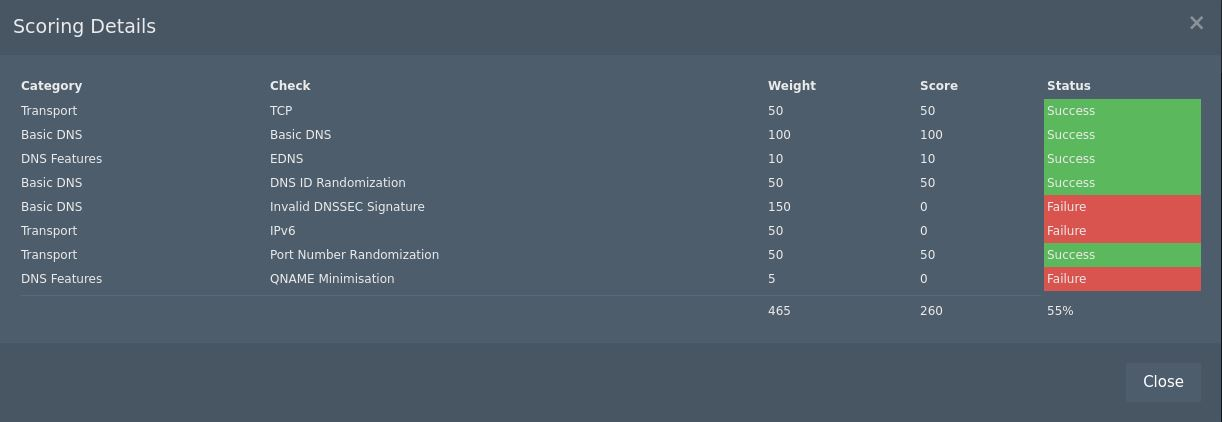
\includegraphics[width=0.6\linewidth]{pics/score_DNS2_before}
		\caption{Name resolver details \textbf{BEFORE}}
	\label{fig:scoredns2before}
\end{figure}
\newpage
\subsubsection{AFTER script}
After the script you have your own domain name resolver and a straight A.
\begin{figure}[H]
	\centering
	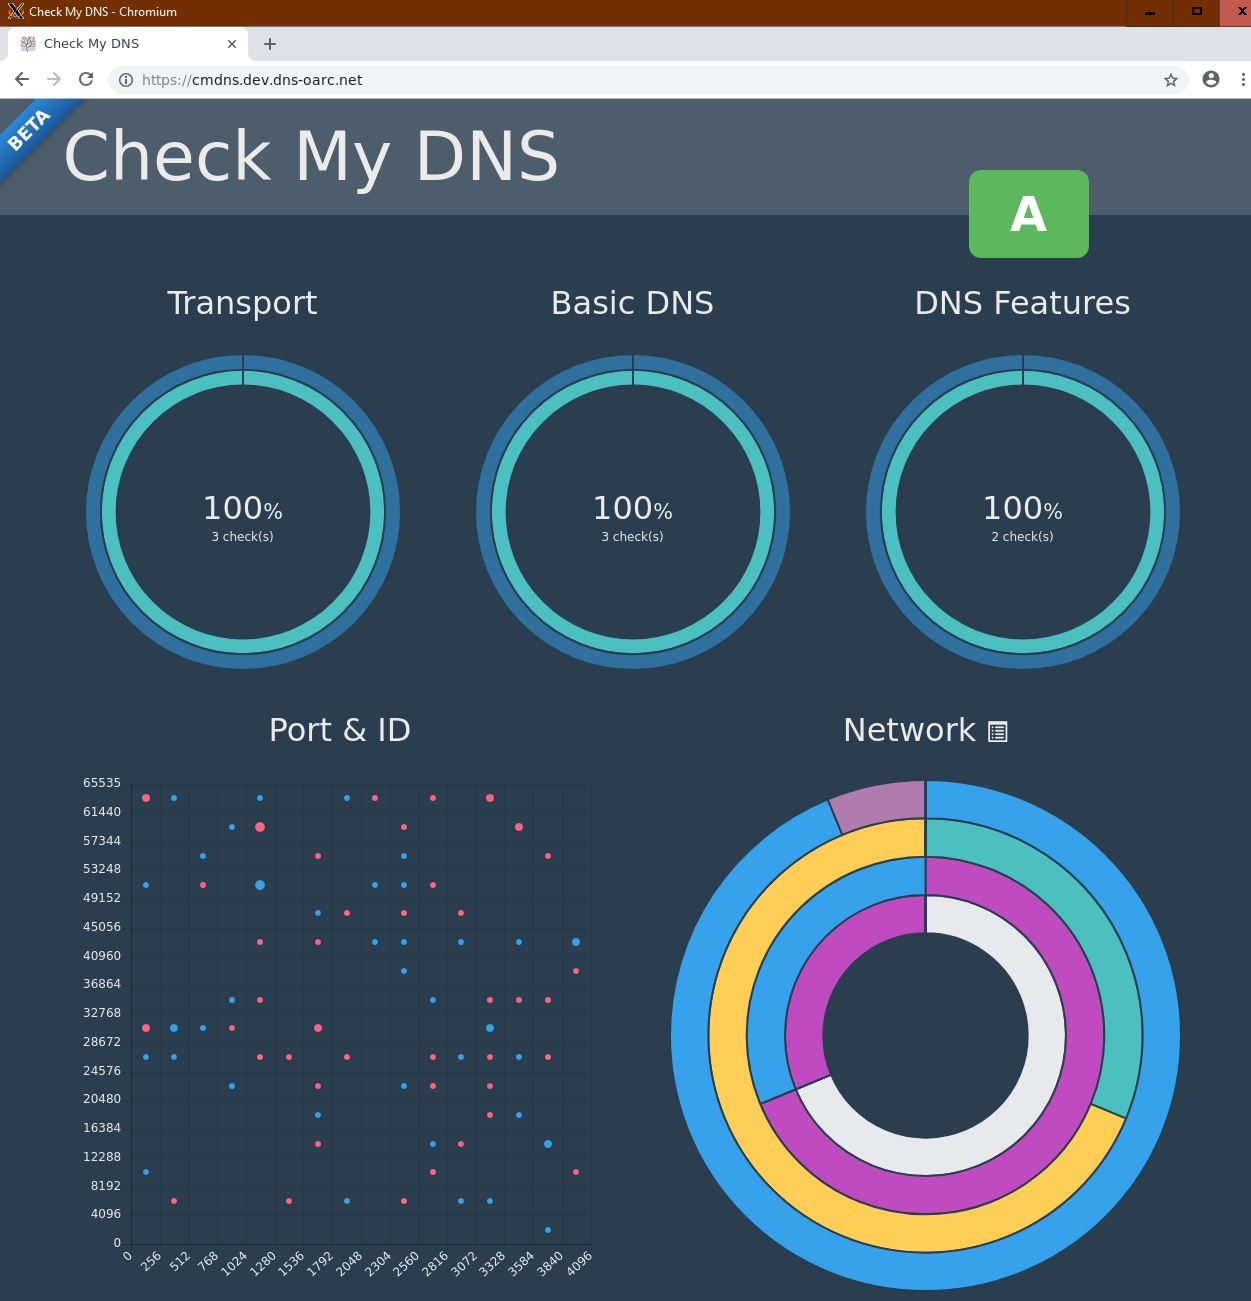
\includegraphics[width=0.9\linewidth]{pics/score_DNS1}
	\label{fig:scoredns1}
		\caption{Name resolver \textbf{AFTER}}
\end{figure}

\begin{figure}[H]
	\centering
	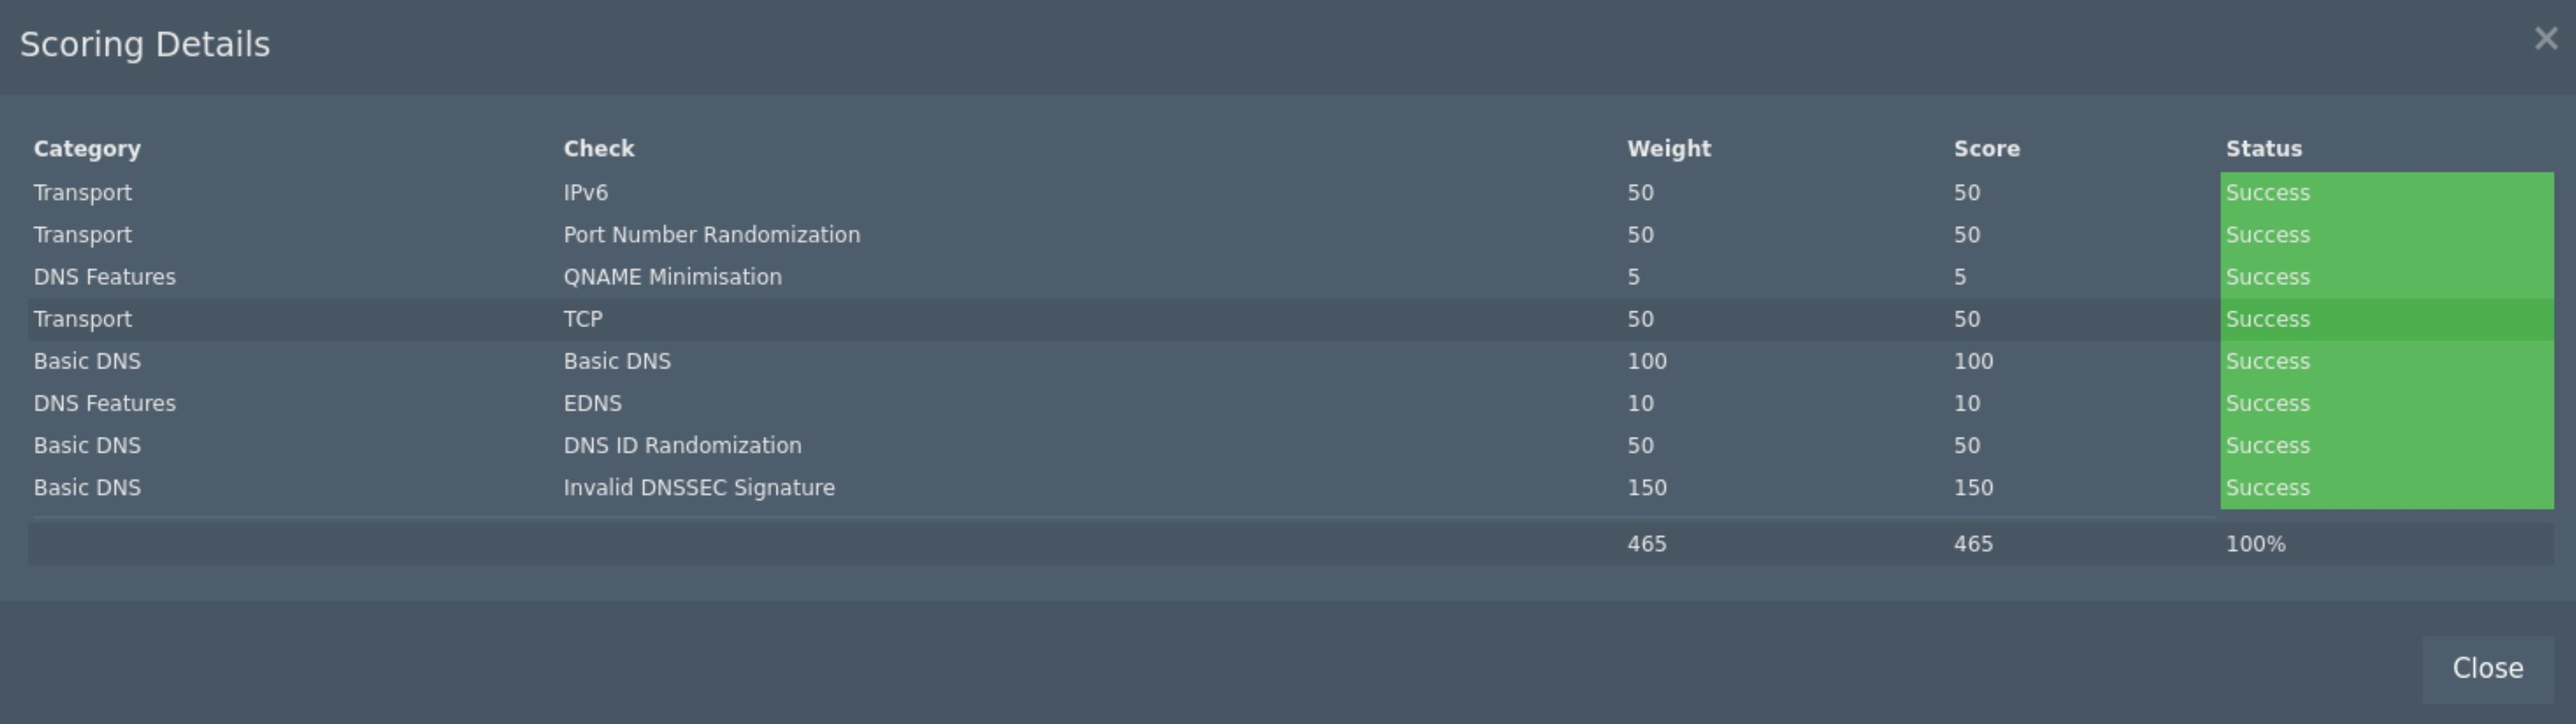
\includegraphics[width=0.9\linewidth]{pics/score_DNS2}
	\label{fig:scoredns2}
			\caption{Name resolver details \textbf{AFTER}}
\end{figure}
\newpage
\subsection{Authoritative DNS}
To setup a authoritative DNS is not easy, and mistakes are easily made. 
\subsubsection{BEFORE script}
Before running the script if you do by hand, misconfiguration can happen. As you can see from \textbf{\textit{https://mxtoolbox.com/}} \cite{mxtoolbox}.
\begin{figure}[H]
	\centering
	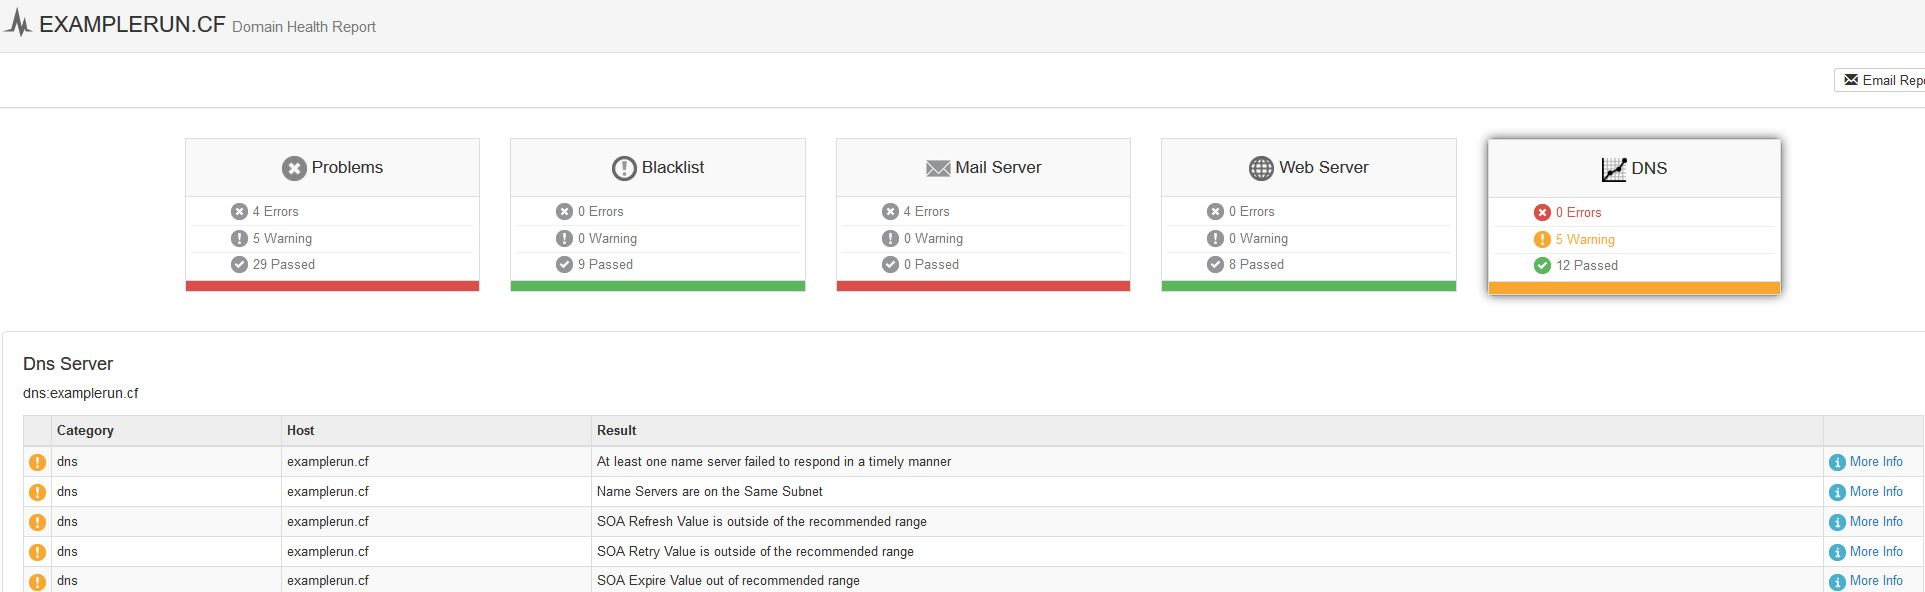
\includegraphics[width=1\linewidth]{pics/mxtool_before_test}
	\label{fig:mxtoolbeforetest}
			\caption{Authoritative DNS test \textbf{BEFORE}}
\end{figure}

\subsubsection{After script}
If you do it with the script, everything will be fine.
\begin{figure}[H]
	\centering
	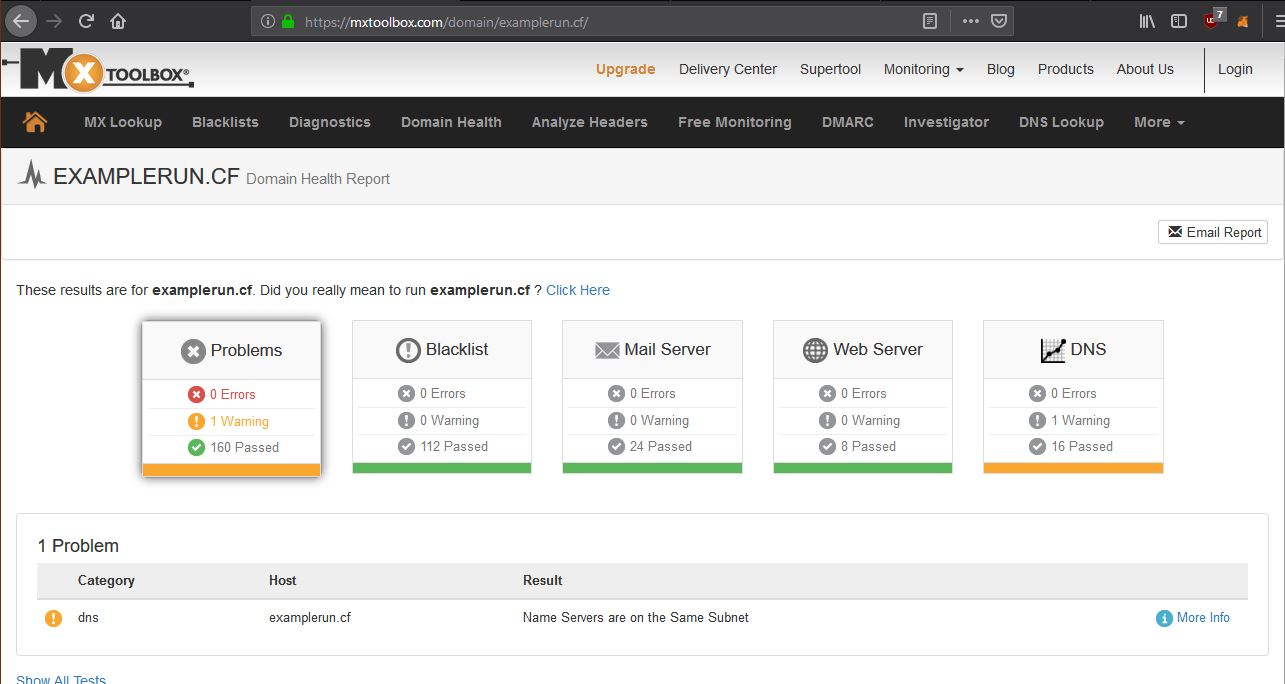
\includegraphics[width=1\linewidth]{pics/mxtool_after_test}
	\label{fig:mxtoolaftertest}
			\caption{Authoritative DNS test \textbf{AFTER}}
\end{figure}
\newpage
